\documentclass{beamer}

\usepackage[T1]{fontenc}
\usepackage[utf8]{inputenc}

\mode<presentation> {
	\usetheme{Rochester}
}

\usepackage{graphicx}
\usepackage{booktabs}
\usepackage{tikz}
\usetikzlibrary{arrows}
\usetikzlibrary{shapes}
\usetikzlibrary{shadows}

%----------------------------------------------------------------------------------------
%	TITLE PAGE
%----------------------------------------------------------------------------------------

\title{\scriptsize{Diplomski rad br. 658} \\ \large{Ocjena učinkovitosti operatora križanja u genetskom programiranju}}
\author{Maja Kontrec}
\institute[FER]{Fakultet elektrotehnike i računarstva}
\date{Srpanj, 2014.}

\definecolor{colourname}{rgb}{.132,.42,.69}
\usecolortheme[named=colourname]{structure}

\begin{document}

\begin{frame}
\titlepage % Print the title page as the first slide
\end{frame}

\begin{frame}
\frametitle{Sadržaj} % Table of contents slide, comment this block out to remove it
\tableofcontents % Throughout your presentation, if you choose to use \section{} and \subsection{} commands, these will automatically be printed on this slide as an overview of your presentation
\end{frame}

%----------------------------------------------------------------------------------------
%	PRESENTATION SLIDES
%----------------------------------------------------------------------------------------

\section{Uvod}

\begin{frame}

\frametitle{Uvod - Genetsko programiranje i operatori križanja} 
\begin{itemize}
\item{genetsko programiranje - optimizacijski postupak koji oponaša prirodnu evoluciju}
\item{križanje - ključan element za napredak algoritma}
\item{velik broj različitih operatora križanja}
\item{odabir operatora križanja - čest problem prilikom postavljanja algoritma}
\end{itemize}

\end{frame}

\section{Operatori križanja}
\subsection{Jednostavno križanje}

%----------------------------------------------------------------------------------------
%	FRAME
%----------------------------------------------------------------------------------------
\begin{frame}

\centering
\frametitle{Jednostavno križanje}
\scalebox{0.65}{

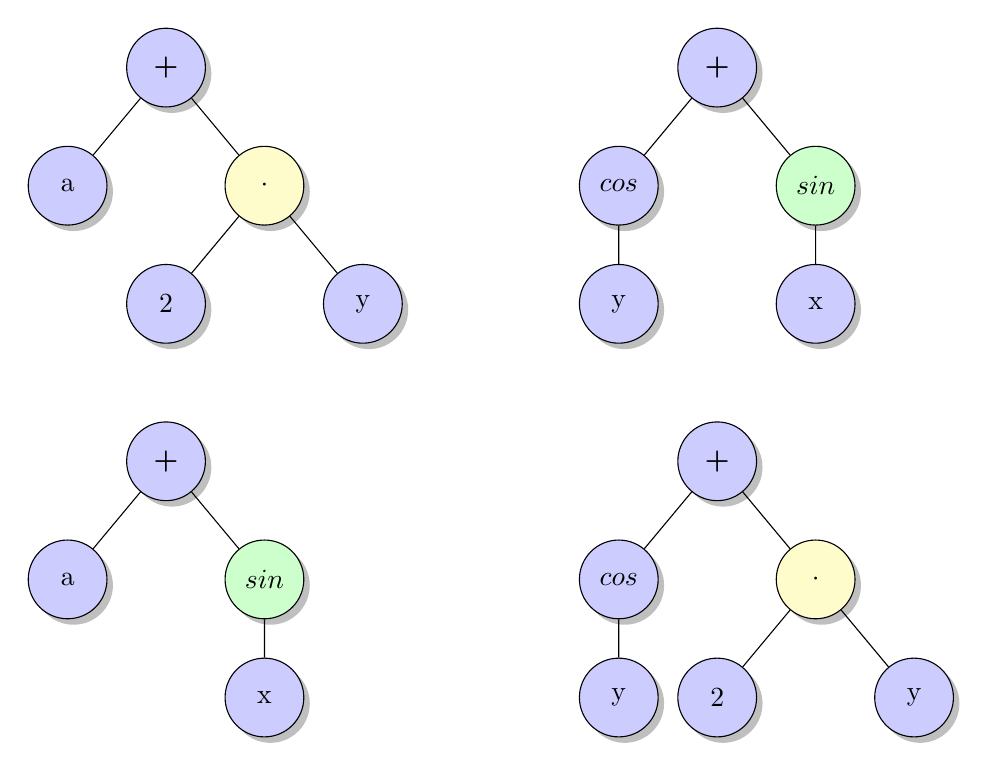
\begin{tikzpicture}
	[sibling distance=25mm, level distance=15mm,
	every node/.style={fill=blue!20,circle,draw,drop shadow, minimum height=1cm}]
	
	
	\node  {\textbf{+}}
    		child {node {a}}
    		child {node [fill=green!20]  {\textbf{$sin$}}
        		child {node  {x}}
      		};

\begin{scope}[xshift=7cm, yshift=0cm]
	\node {\textbf{+}}
    		child {node {$cos$}
        		child {node {y}}
      		}
     		child {node [fill=yellow!20]  {\textbf{$\cdot$}}
        		child {node {2}}
        		child {node {y}}
      		};
\end{scope}

\begin{scope}[xshift=0cm, yshift=5cm]

	\node {\textbf{+}}
    		child {node {a}}
    		child {node [fill=yellow!20]  {\textbf{$\cdot$}}
        		child {node {2}}
        		child {node {y}}
      		};
\end{scope}

\begin{scope}[xshift=7cm, yshift=5cm]
	\node {\textbf{+}}
    		child {node {$cos$}
        		child {node {y}}
      		}
    		child {node [fill=green!20] {\textbf{$sin$}}
			child {node {x}}};
\end{scope}

\end{tikzpicture}
}


\begin{itemize}
\item{nasumičan odabir točke prekida u svakom roditelju}
\item{spajanje dva podstabla ispod ili iznad točke križanja}
\end{itemize}
\end{frame}


%----------------------------------------------------------------------------------------
%	FRAME
%----------------------------------------------------------------------------------------

\subsection{Križanje s jednom točkom prekida}
\begin{frame}
\centering
\frametitle{Križanje s jednom točkom prekida}

\scalebox{0.5}{

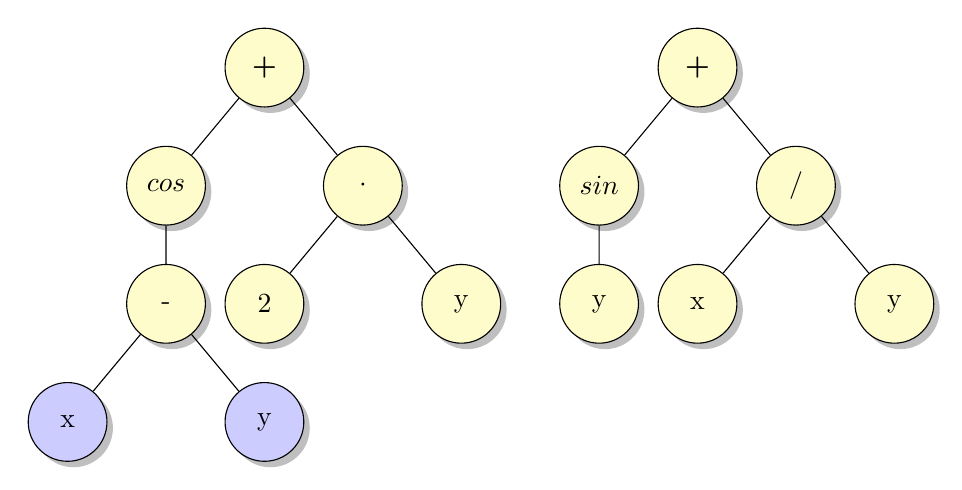
\begin{tikzpicture}
	[sibling distance=25mm, level distance=15mm,
	every node/.style={fill=blue!20,circle,draw,drop shadow, minimum height=1cm}]

\begin{scope}[xshift=0cm]

	\node  [fill=yellow!20]  {\textbf{+}}
    		child {node [fill=yellow!20]  {$cos$}
    			child {node  [fill=yellow!20] {-}
    				child {node{x}}
    				child {node{y}}
    			}
    		}
    		child {node [fill=yellow!20]  {\textbf{$\cdot$}}
        		child {node [fill=yellow!20]  {2}}
        		child {node [fill=yellow!20]  {y}}
	};
\end{scope}

\begin{scope}[xshift=5.5cm]
	\node  [fill=yellow!20]  {\textbf{+}}
    		child {node  [fill=yellow!20] {$sin$}
        		child {node  [fill=yellow!20] {y}}
      		}
    		child {node [fill=yellow!20] {\textbf{$/$}}
			child {node [fill=yellow!20]  {x}}
			child {node [fill=yellow!20]  {y}}	
		};
\end{scope}

\end{tikzpicture}
}

\begin{itemize}
\item{odabir točke prekida iz zajedničkog područja}
\end{itemize}

\scalebox{0.5}{

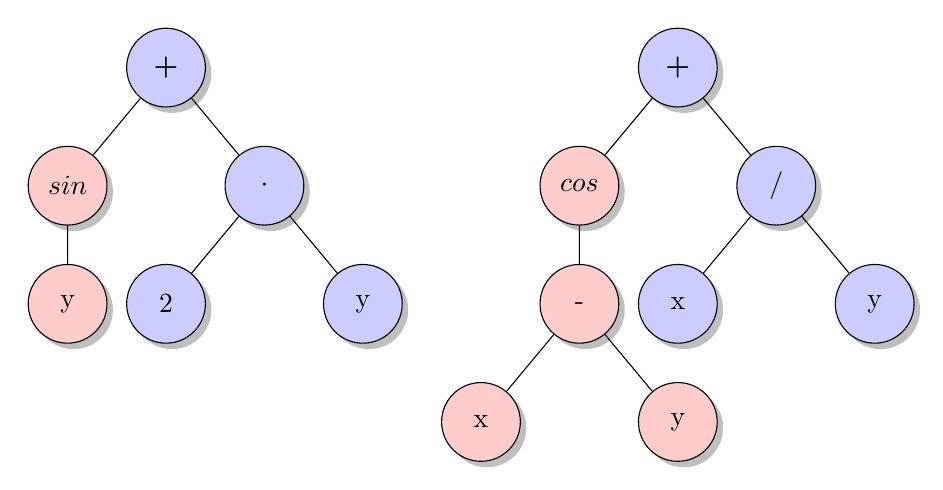
\begin{tikzpicture}
	[sibling distance=25mm, level distance=15mm,
	every node/.style={fill=blue!20,circle,draw,drop shadow, minimum height=1cm}]

\begin{scope}[xshift=0cm]

	\node {\textbf{+}}
    		child {node [fill=red!20]  {$sin$}
    				child {node [fill=red!20]{y}}
    		}
    		child {node {\textbf{$\cdot$}}
        		child {node{2}}
        		child {node {y}}
	};
\end{scope}

\begin{scope}[xshift=6.5cm]
	\node   {\textbf{+}}
    		child {node [fill=red!20] {$cos$}
    			child {node [fill=red!20]{-}
    				child {node [fill=red!20]{x}}
    				child {node [fill=red!20]{y}}
    			}
    		}
    		child {node {\textbf{$/$}}
			child {node  {x}}
			child {node  {y}}	
	};
\end{scope}

\end{tikzpicture}
}

\begin{itemize}
\item{spajanje dva podstabla ispod ili iznad točke prekida}
\end{itemize}
\end{frame}


%----------------------------------------------------------------------------------------
%	FRAME
%----------------------------------------------------------------------------------------

\subsection{Križanje s očuvanjem konteksta}
\begin{frame}
\frametitle{Križanje s očuvanjem konteksta}
\centering

\begin{itemize}
\item{koordinate čvorova stabla}
\end{itemize}
\scalebox{0.4}{
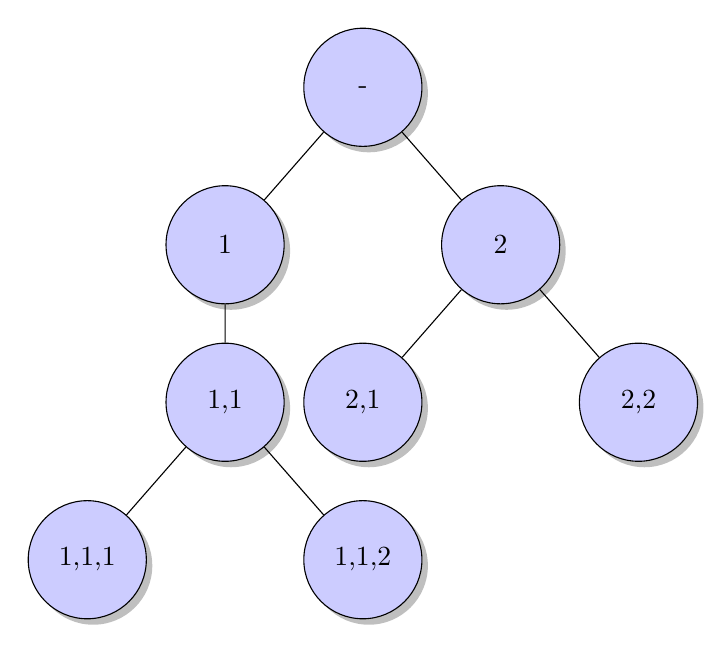
\begin{tikzpicture}
	[sibling distance=35mm, level distance=20mm,
	every node/.style={fill=blue!20,circle,draw,drop shadow, minimum height=1.5cm}]
	\node   {-}
    		child {node  {1}
    			child {node {1,1}
    				child {node{1,1,1}}
    				child {node{1,1,2}}
    			}
    		}
    		child {node {2}
        		child {node  {2,1}}
        		child {node {2,2}}
      		};

\end{tikzpicture}
}
%\end{frame}

%----------------------------------------------------------------------------------------
%	FRAME
%----------------------------------------------------------------------------------------
%\begin{frame}
%\frametitle{Križanje s očuvanjem konteksta}
\begin{itemize}
\item{\textbf{križanje s jakim očuvanjem konteksta} - križanje podstabala koja imaju potpuno jednake koordinate korijena}
\item{ \textbf{križanje sa slabim očuvanjem konteksta}
	\begin{itemize}
	\item{ako su $T1$ i $T2$ važeći odabiri podstabala za križanje s jakim očuvanjem konteksta, 		tada su $T1$ i $T2' \subseteq T2$ važeći odabiri podstabala za križanje sa slabim očuvanjem 		konteksta}
	
	\end{itemize}
}
\end{itemize}

\end{frame}

%----------------------------------------------------------------------------------------
%	FRAME
%----------------------------------------------------------------------------------------
\subsection{Križanje pravedno s obzirom na veličinu}
\begin{frame}
\frametitle{Križanje pravedno s obzirom na veličinu}
\centering
\scalebox{0.45}{

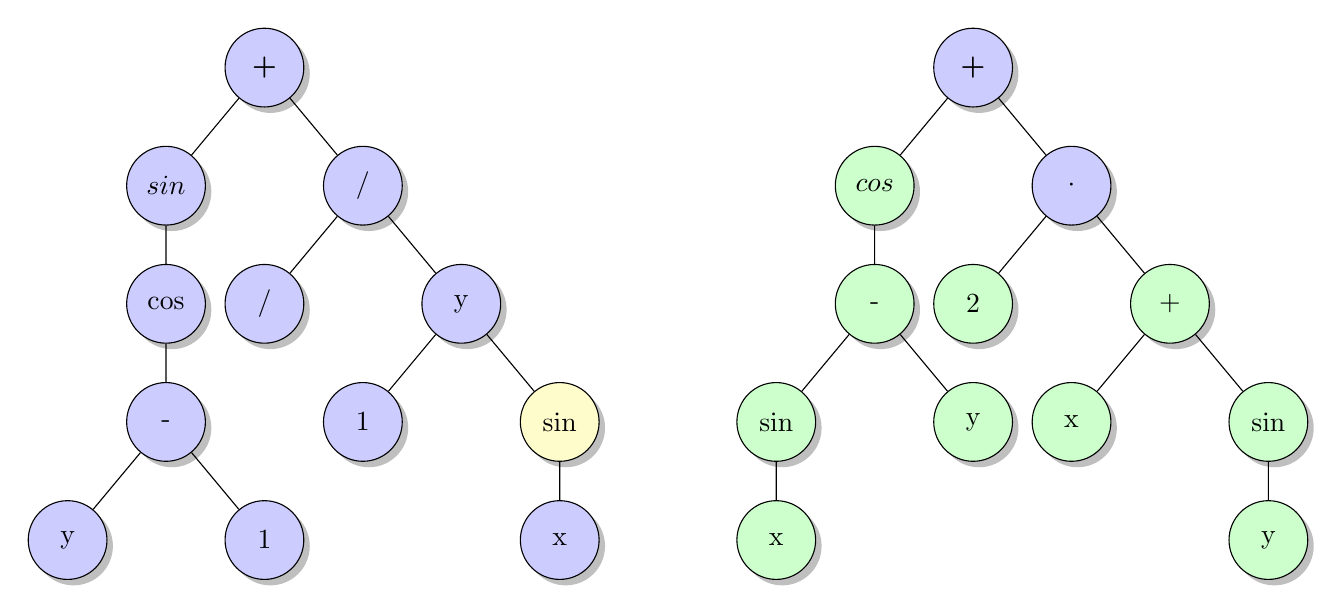
\begin{tikzpicture}
	[sibling distance=25mm, level distance=15mm,
	every node/.style={fill=blue!20,circle,draw,drop shadow, minimum height=1cm}]

\begin{scope}[xshift=0cm]
\node  {\textbf{+}}
    		child {node {$sin$}
        		child {node {cos}
        			child{node {-}
        				child {node {y}}
        				child {node {1}}
        			}
        		}
      		}
    		child {node  {\textbf{$/$}}
			child {node {/}}
			child {node {y}
				child {node {1}}
				child {node [fill=yellow!20]  {sin}
					child {node {x}}
				}
			}	
		};
	
\end{scope}

\begin{scope}[xshift=9cm]
	\node   {\textbf{+}}
    		child {node [fill=green!20] {$cos$}
    			child {node [fill=green!20]   {-}
    				child {node [fill=green!20] {sin}
    					child {node [fill=green!20] {x}}
    				}
    				child {node [fill=green!20] {y}}
    			}
    		}
    		child {node {\textbf{$\cdot$}}
        		child {node [fill=green!20] {2}}
        		child {node [fill=green!20]  {+}
        			child {node [fill=green!20] {x}}
        			child {node [fill=green!20] {sin}
        				child {node [fill=green!20] {y}}
        			}
        		}
	};
\end{scope}

\end{tikzpicture}
}


\begin{itemize}
\item{inačica jednostavnog križanja}
\item{sprječavanje prekomjernog rasta novih jedinki u samom postupku križanja}
\item{odabir nezavršnog čvora kao točke prekida s vjerojatnošću od 0.9}
\item{nasumičan odabir točke prekida $b$ u prvom roditelju}
\item{u drugom roditelju pronalaze se točke prekida koje su korijen podstabala veličine ne veće od $1 + 2 \cdot s$, gdje je $s$ veličina podstabla u prvom roditelju čiji je korijen $b$}
\end{itemize}
\end{frame}


%----------------------------------------------------------------------------------------
%	FRAME
%----------------------------------------------------------------------------------------
\subsection{Uniformno križanje}
\begin{frame}
\frametitle{Uniformno križanje}
\centering

\begin{itemize}
\item{zajedničko područje roditelja}
\end{itemize}
\scalebox{0.5}{

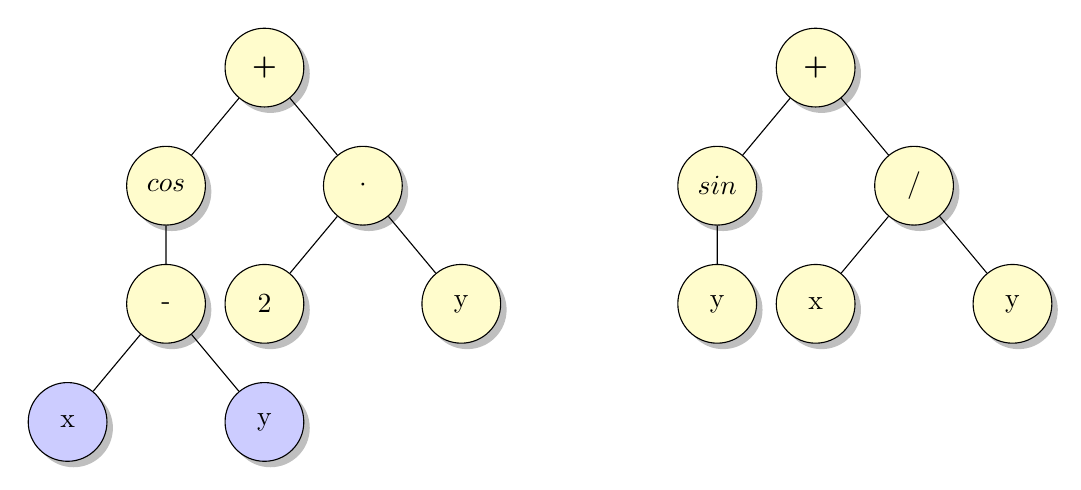
\begin{tikzpicture}
	[sibling distance=25mm, level distance=15mm,
	every node/.style={fill=blue!20,circle,draw,drop shadow, minimum height=1cm}]

\begin{scope}[xshift=0cm]

	\node  [fill=yellow!20]  {\textbf{+}}
    		child {node [fill=yellow!20]  {$cos$}
    			child {node  [fill=yellow!20] {-}
    				child {node{x}}
    				child {node{y}}
    			}
    		}
    		child {node [fill=yellow!20]  {\textbf{$\cdot$}}
        		child {node [fill=yellow!20]  {2}}
        		child {node [fill=yellow!20]  {y}}
      		};
\end{scope}

\begin{scope}[xshift=7cm]
	\node  [fill=yellow!20]  {\textbf{+}}
    		child {node  [fill=yellow!20] {$sin$}
        		child {node  [fill=yellow!20] {y}}
      		}
    		child {node [fill=yellow!20] {\textbf{$/$}}
			child {node [fill=yellow!20]  {x}}
			child {node [fill=yellow!20]  {y}}	
		};
\end{scope}

\end{tikzpicture}
}
\begin{itemize}
\item{ravnomjeran odabir čvorova iz dva roditeljska stabla}
\end{itemize}
\scalebox{0.5}{

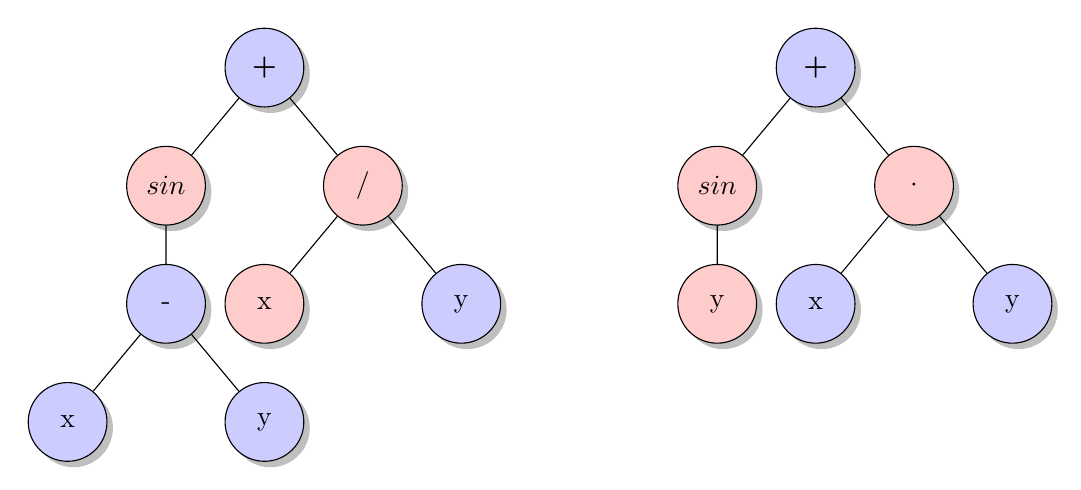
\begin{tikzpicture}
	[sibling distance=25mm, level distance=15mm,
	every node/.style={fill=blue!20,circle,draw,drop shadow, minimum height=1cm}]

\begin{scope}[xshift=0cm]

	\node {\textbf{+}}
    		child {node [fill=red!20]  {$sin$}
    				child {node{-}
    					child {node {x}}
    					child {node {y}}
    			}
    		}
    		child {node  [fill=red!20] {\textbf{$/$}}
        		child {node [fill=red!20]  {x}}
        		child {node {y}}
	};
\end{scope}

\begin{scope}[xshift=7cm]
	\node   {\textbf{+}}
    		child {node  [fill=red!20] {$sin$}
        		child {node  [fill=red!20] {y}}
      		}
    		child {node  [fill=red!20]  {\textbf{$\cdot$}}
			child {node  {x}}
			child {node  {y}}	
	};
\end{scope}

\end{tikzpicture}
}
\end{frame}


%----------------------------------------------------------------------------------------
%	FRAME
%----------------------------------------------------------------------------------------
\subsection{Homologno križanje}
\begin{frame}
\frametitle{Homologno križanje}
\begin{itemize}
\item{uzima u obzir \textbf{veličinu i poziciju} podstabala prilikom križanja}
\item{inačica križanja pravednog s obzirom na veličinu}

\begin{figure}[H]
	\centering
	\includegraphics[scale=0.3]{./slike/crxHomo.png}
\end{figure}
\item{u drugom roditelju između kandidata koji zadovoljavaju veličinski kriterij prednost imaju podstabla s korijenom slične pozicije kao točka prekida u prvom roditelju}
\end{itemize}

\end{frame}


%----------------------------------------------------------------------------------------
%	FRAME
%----------------------------------------------------------------------------------------
\subsection{Determinističko križanje}
\begin{frame}
\frametitle{Determinističko križanje}
\begin{itemize}
\item{primjenjivo isključivo na probleme simboličke regresije}

\item{nasumičan odabir točke prekida u prvom roditelju}
\item{u drugom roditelju odabire se točka prekida takva da funkcijska udaljenost između nje i točke prekida u prvom roditelju bude minimalna}
\item{funkcijska udaljenost između dva čvora $i$ i $j$ jednaka je
\begin{equation} 
 \large{ d_{i,j} = \frac{1}{2} (|max_i - max_j| + |min_i - min_j|), }
\end{equation}
gdje su $max_u$ i $min_u$ maksimalna, odnosno, minimalna vrijednost čvora $u$ koju on poprima na svim ispitnim primjerima u skupu za učenje}
\end{itemize}
\end{frame}


%----------------------------------------------------------------------------------------
%	FRAME
%----------------------------------------------------------------------------------------
\begin{frame}
\frametitle{Determinističko križanje}
\centering

\begin{itemize}
\item{primjer: $x = 1, y = 1$}
\end{itemize}

\scalebox{0.7}{
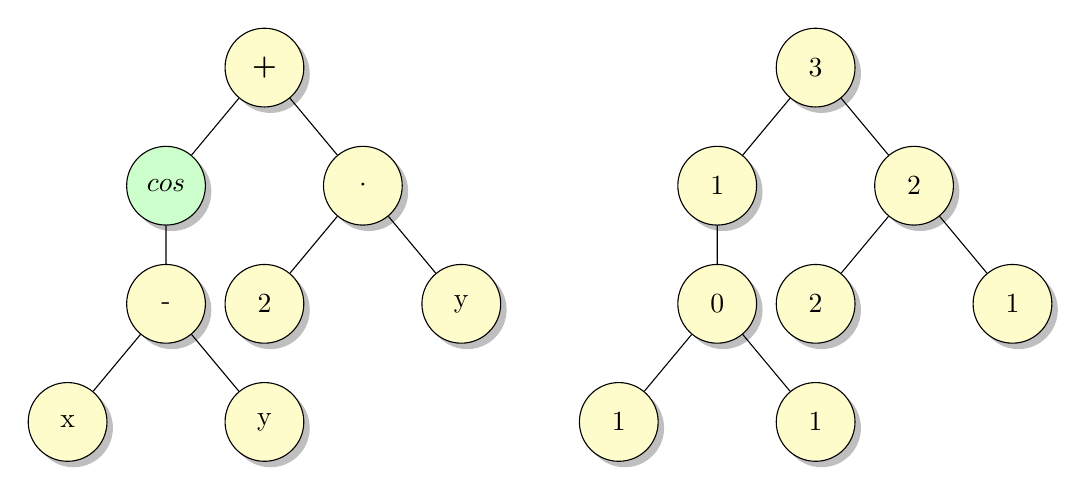
\begin{tikzpicture}
	[sibling distance=25mm, level distance=15mm,
	every node/.style={fill=yellow!20,circle,draw,drop shadow, minimum height=1cm}]

\begin{scope}[xshift=0cm]
	\node {\textbf{+}}
    		child {node [fill=green!20] {$cos$}
    			child {node {-}
    				child {node{x}}
    				child {node{y}}
    			}
    		}
    		child {node  {\textbf{$\cdot$}}
        		child {node {2}}
        		child {node {y}}
      		};
\end{scope}

\begin{scope}[xshift=7cm]
	\node {3}
    		child {node {$1$}
    			child {node  [fill=yellow!20] {0}
    				child {node{1}}
    				child {node{1}}
    			}
    		}
    		child {node  {2}
        		child {node {2}}
        		child {node {1}}
      		};
\end{scope}

\end{tikzpicture}
}

\begin{itemize}
\item{primjerice, za čvor označen zelenom bojom, vrijednost $v$ za dane $x$ i $y$ računa se kao: $v = cos(x-y) = cos (1-1) = cos (0) = 1$}
\end{itemize}

\end{frame}

%----------------------------------------------------------------------------------------
%	FRAME
%----------------------------------------------------------------------------------------
\subsection{Probabilističko križanje}
\begin{frame}
\frametitle{Probabilističko križanje}
\begin{itemize}
\item{probabilistička inačica determinističkog križanja}
\item{primjenjivo isključivo na probleme simboličke regresije}
\item{prilikom odabira točke prekida u drugom roditelju, izračunavaju se vjerojatnosti odabira pojedinog čvora za drugu točku prekida
\begin{equation} 
 \large{ d '_{i,j} = \frac{d_{i,j}}{\sum_{k=1}^{s} d_{i,k}} }
\end{equation}
\begin{equation} 
\label{prob}
 \large{ p_{i,j} = \frac{1 - d '_{i,j}}{\sum_{k=1}^{s} (1 - d '_{i,k})} }
\end{equation}}
\item{ovime, funkcijski bliži čvorovi drugog roditelja imaju veću vjerojatnost odabira}
\end{itemize}
\end{frame}



%----------------------------------------------------------------------------------------
%	FRAME
%----------------------------------------------------------------------------------------
\subsection{Semantičko križanje}
\begin{frame}
\frametitle{Semantičko križanje}
\begin{itemize}
\item{\textcolor{colourname}{\textbf{logičke funkcije:}}

 \begin{equation} 
 \large{ D = (T1 \cdot TR) +   ((1-TR) \cdot T2) }
\end{equation}
}
\item{\textcolor{colourname}{\textbf{simbolička regresija:}}
 \begin{equation} 
 \large{ D = (T1 \cdot TR) +   ((1-TR) \cdot T2), }
\end{equation}

 gdje je $TR$ nasumično generirana jedinka, $T1$ i $T2$ roditelji, a $D$ dijete
}
\item{\textcolor{colourname}{\textbf{programi:}}
 \begin{equation} 
 \large{ D = \textbf{IF}(CONDR) \textbf{THEN} (T1) \textbf{ELSE} (T2),}
\end{equation}
gdje je $CONDR$ nasumično generiran program čiji je izlaz interpretiran kao logička vrijednost
}
\end{itemize}

\end{frame}


%----------------------------------------------------------------------------------------
%	FRAME
%----------------------------------------------------------------------------------------
\section{Ispitivanja}
\subsection{Problemi za ispitivanje}
\begin{frame}
\frametitle{Problemi za ispitivanje}
\begin{itemize}
\item{logičke funkcije
	\begin{itemize}
	\item{6 i 11 - multipleksor problem}
	\item{evolucija kriptografski sigurnih logičkih funkcija (dvije inačice)}
	\end{itemize}
}
\item{simbolička regresija
	\begin{itemize}
	\item{klasična simbolička regresija (šest različitih izraza)}
	\item{evolucija funkcije prioriteta za uporabu unutar pravila raspoređivanja}
	\end{itemize}
}
\item{programi
	\begin{itemize}
	\item{problem umjetnog mrava}
	\end{itemize}
}

\end{itemize}
\end{frame}


\subsection{Rezultati}


%----------------------------------------------------------------------------------------
%	FRAME
%----------------------------------------------------------------------------------------
\begin{frame}
\frametitle{Ispitivanja}
\begin{itemize}
\item{usporedba isključivog korištenja jednog operatora križanja}
\item{u svakom eksperimentu svi parametri osim operatora križanja su konstanti}
\item{zbog eksponencijalnog rasta novih jedinki, semantičko križanje korišteno je u kombinaciji s jednostavnim križanjem u omjeru 1:9}
\end{itemize}

\end{frame}
%----------------------------------------------------------------------------------------
%	FRAME
%----------------------------------------------------------------------------------------
\begin{frame}
\frametitle{6 - multipleksor (minimizacija)}


\begin{figure}[!htb]
\minipage{0.62\textwidth}
\begin{figure}[H]
	\centering
	\includegraphics[trim=3cm 6cm 0cm 3.5cm, scale=0.3]{./boxPlots/mux6.eps}
\end{figure}
\endminipage
\minipage{0.65\textwidth}
\scalebox{0.59}{
    \centering
    \begin{tabular}{| l | l | l |}
    \hline
    \textbf{operator}  & \textbf{medijan dobrote} & \textbf{rang}\\ \hline
    simple & 4 & 1\\ \hline
    one point & 6 & 6\\ \hline
    context preserved & 4 & 1\\ \hline
    size fair & 4 & 1\\ \hline
    uniform & 4 & 1\\ \hline
    homologous & 4 & 1\\ \hline
    semantic & 14.5 & 7\\ \hline
    \end{tabular}
}
\endminipage
\end{figure}

\begin{itemize}
\item{veličina populacije = 400}
\item{broj generacija = 15}
\item{faktor mutacije = 0.4}
\item{nezavršni znakovi: \textit{AND, OR, NOT, IF}}
\item{završni znakovi: \textit{$a_0, a_1, d_0, d_1, d_2, d_3$}}
\end{itemize}
\end{frame}


%----------------------------------------------------------------------------------------
%	FRAME
%----------------------------------------------------------------------------------------
\begin{frame}
\frametitle{11 - multipleksor (minimizacija)}


\begin{figure}[!htb]
\minipage{0.627\textwidth}
\begin{figure}[H]
	\centering
	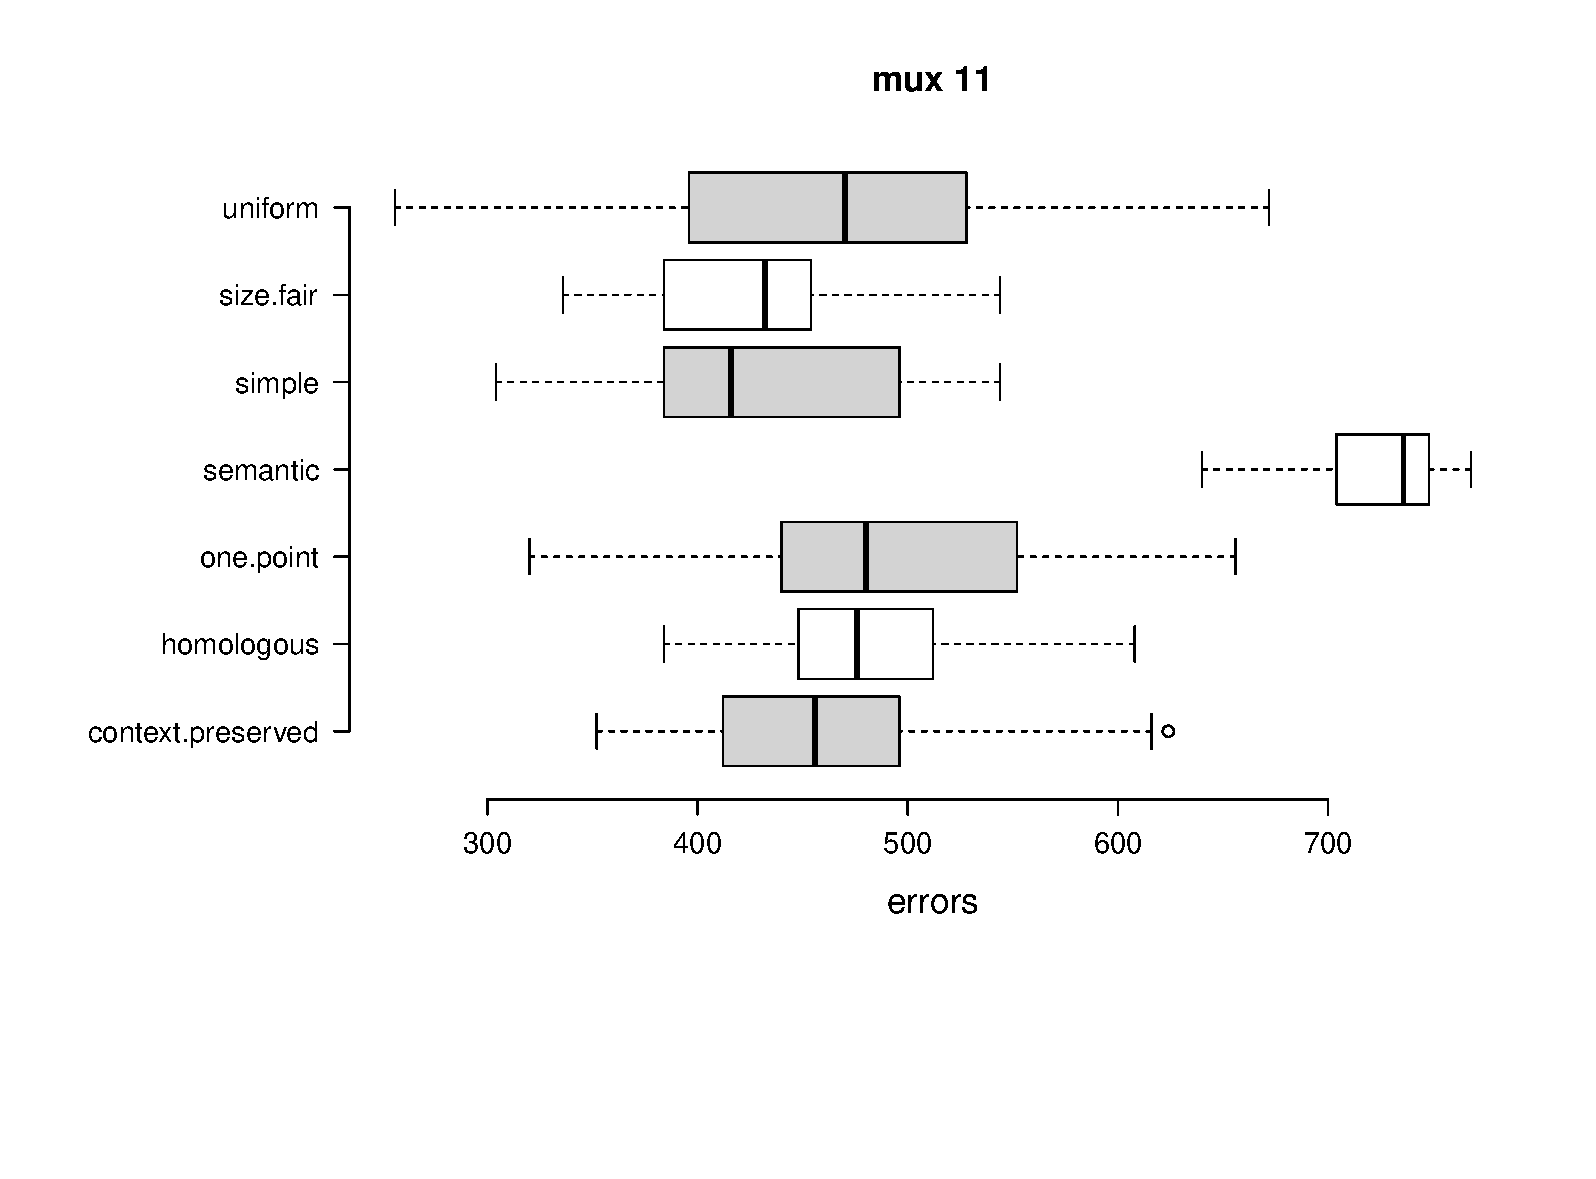
\includegraphics[trim=3cm 6cm 0cm 3.5cm, scale=0.3]{./boxPlots/mux11.eps}
\end{figure}
\endminipage
\minipage{0.65\textwidth}
\scalebox{0.59}{
    \centering
    \begin{tabular}{| l | l | l |}
    \hline
    \textbf{operator} & \textbf{medijan dobrote} & \textbf{rang}\\ \hline
    simple & 416 &1\\ \hline
    one point & 480 & 6\\ \hline
    context preserved & 456 & 3\\ \hline
    size fair & 432 & 2\\ \hline
    uniform & 470 & 4\\ \hline
    homologous & 476 & 5\\ \hline
    semantic & 736 & 7\\ \hline
    \end{tabular}
}
\endminipage
\end{figure}

\begin{itemize}
\item{veličina populacije = 200}
\item{broj evaluacija = 8000}
\item{faktor mutacije = 0.3}
\item{nezavršni znakovi: \textit{AND, OR, NOT, IF}}
\item{završni znakovi: \textit{$a_0, a_1, a_2, d_0, d_1, d_2, d_3, d_4, d_5, d_6, d_7$}}
\end{itemize}
\end{frame}

%----------------------------------------------------------------------------------------
%	FRAME
%----------------------------------------------------------------------------------------
\begin{frame}
\frametitle{Evolucija kriptografski sigurnih logičkih funkcija - inačica 1
 (maksimizacija)}


\begin{figure}[!htb]
\minipage{0.6\textwidth}
\begin{figure}[H]
	\centering
	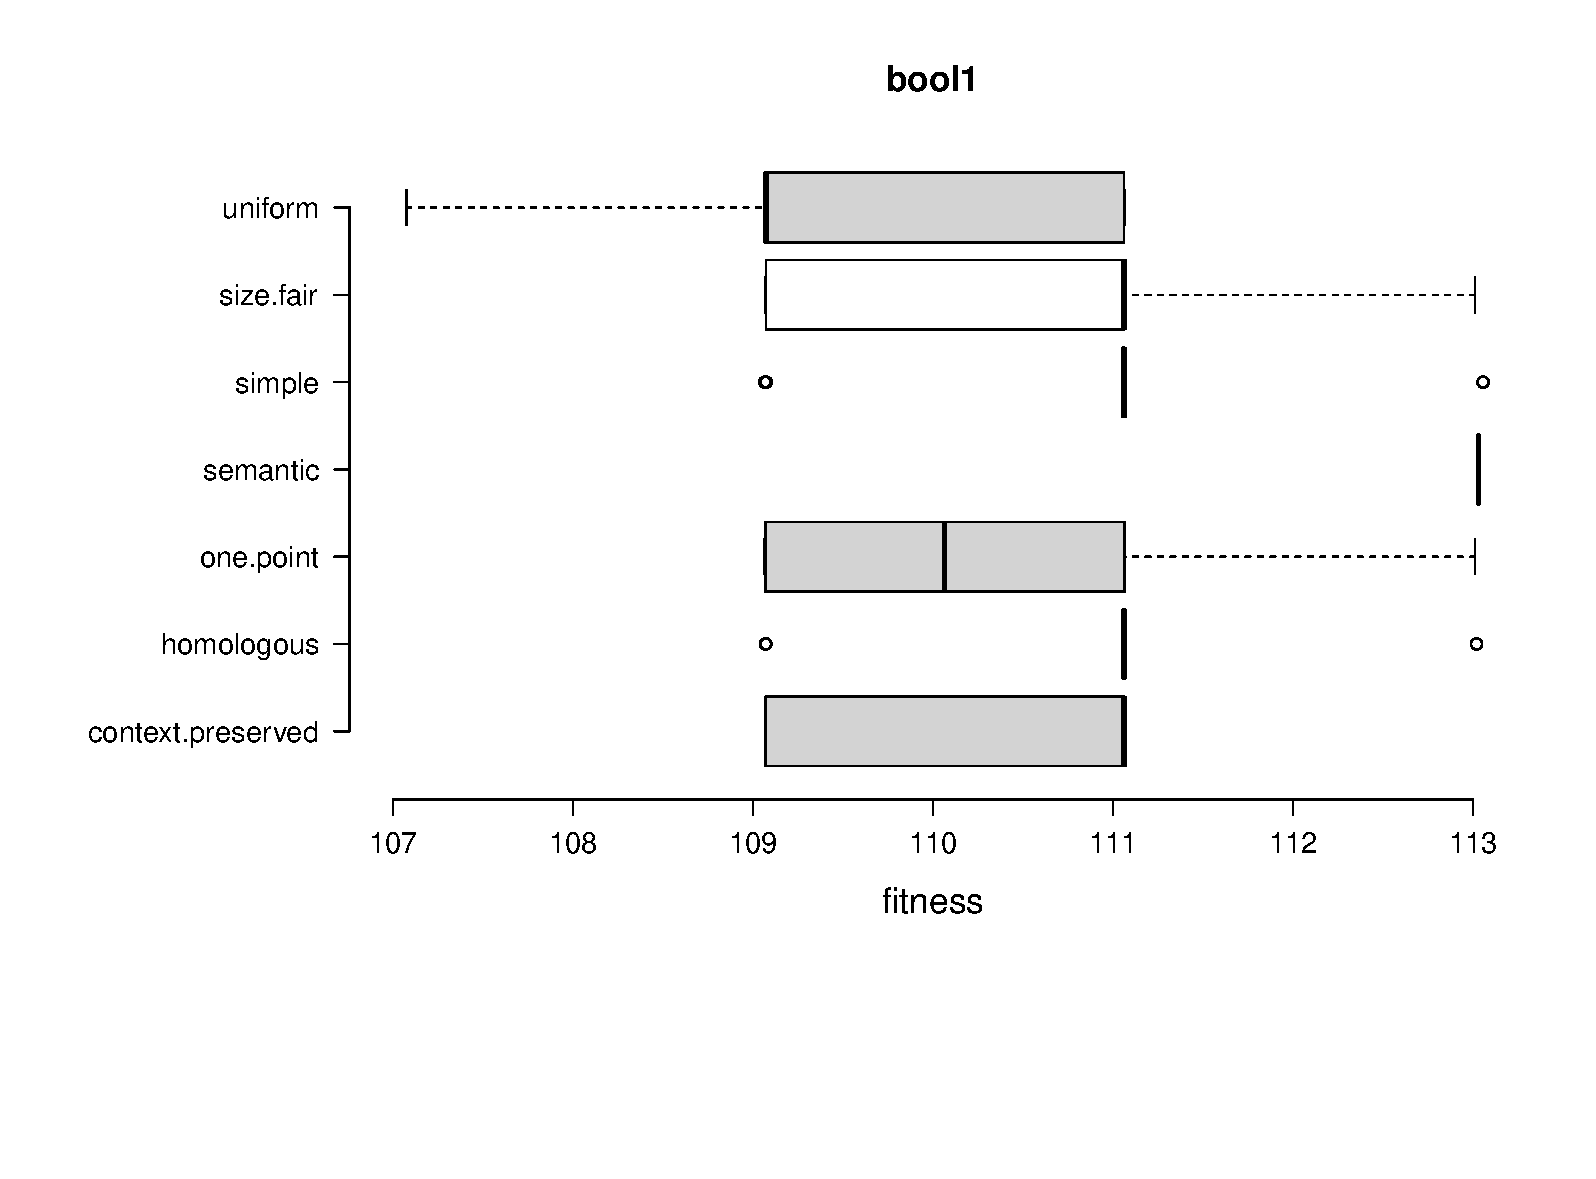
\includegraphics[trim=3cm 5.5cm 0cm 3.5cm, scale=0.27]{./boxPlots/bool1.eps}
\end{figure}
\endminipage
\minipage{0.65\textwidth}
\scalebox{0.59}{
    \centering   
    \begin{tabular}{| l | l | l |}
    \hline
    \textbf{operator} & \textbf{medijan dobrote} & \textbf{rang}\\ \hline
    simple & 111.061 & 3\\ \hline
    one point & 110.0645 & 6\\ \hline
    context preserved & 111.06 & 5\\ \hline
    size fair & 111.061 & 3\\ \hline
    uniform & 109.071 & 7\\ \hline
    homologous & 111.062 & 2\\ \hline
    semantic & 113.031& 1\\ \hline
    \end{tabular}
    
}
\endminipage
\end{figure}

\begin{itemize}
\item{dobrota u obzir uzima balans i nelinearnost evoluirane funkcije}
\item{veličina populacije = 250}
\item{broj evaluacija = 3750}
\item{faktor mutacije = 0.3}
\item{nezavršni znakovi: \textit{AND OR NOT IF XOR}}
\item{završni znakovi: \textit{$v_0, v_1, v_2, v_3, v_4, v_5, v_6, v_7$}}
\end{itemize}
\end{frame}

%----------------------------------------------------------------------------------------
%	FRAME
%----------------------------------------------------------------------------------------
\begin{frame}
\frametitle{Evolucija kriptografski sigurnih logičkih funkcija - inačica 4
 (maksimizacija)}


\begin{figure}[!htb]
\minipage{0.59\textwidth}
\begin{figure}[H]
	\centering
	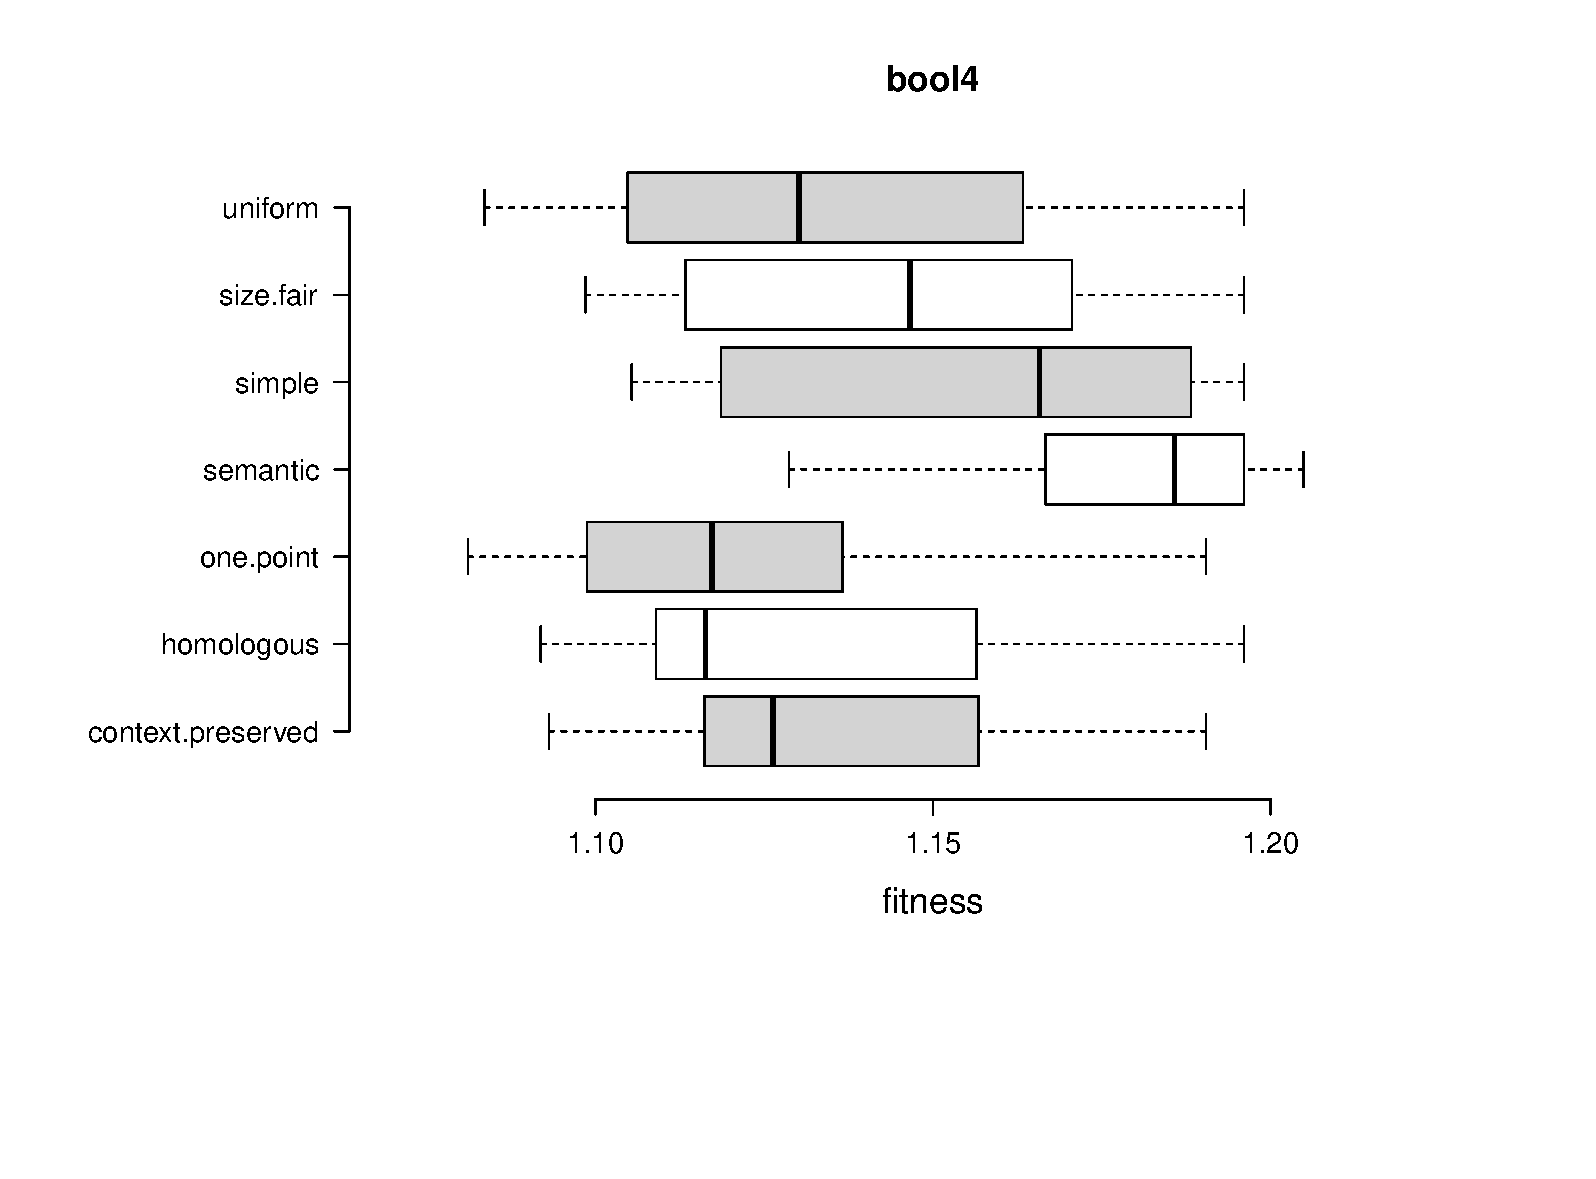
\includegraphics[trim=3cm 5.5cm 0cm 3.5cm, scale=0.3]{./boxPlots/bool4.eps}
\end{figure}

\endminipage
\minipage{0.59\textwidth}
\scalebox{0.59}{
    \centering   
       \begin{tabular}{| l | l | l |}
    \hline
    \textbf{operator} & \textbf{medijan dobrote} & \textbf{rang}\\ \hline
    simple & 1.16581 & 2\\ \hline
    one point & 1.11728 & 6\\ \hline
    context preserved & 1.12635 & 5\\ \hline
    size fair & 1.14657 & 3\\ \hline
    uniform & 1.130145 & 4\\ \hline
    homologous & 1.1163 & 7\\ \hline
    semantic & 1.185785 & 1\\ \hline
    \end{tabular}    
}
\endminipage
\end{figure}

\begin{itemize}
\item{dobrota u obzir uzima transparentnost i balansiranost funkcije}
\item{veličina populacije = 250}
\item{broj evaluacija = 3750}
\item{faktor mutacije = 0.3}
\item{nezavršni znakovi: \textit{AND, OR, NOT, IF, XOR}}
\item{završni znakovi: \textit{$v_0, v_1, v_2, v_3, v_4, v_5, v_6, v_7$}}
\end{itemize}
\end{frame}


%----------------------------------------------------------------------------------------
%	FRAME
%----------------------------------------------------------------------------------------
\begin{frame}
\frametitle{Simbolička regresija 1 (minimizacija)}


\begin{figure}[!htb]
\minipage{0.65\textwidth}
\begin{figure}[H]
	\centering
	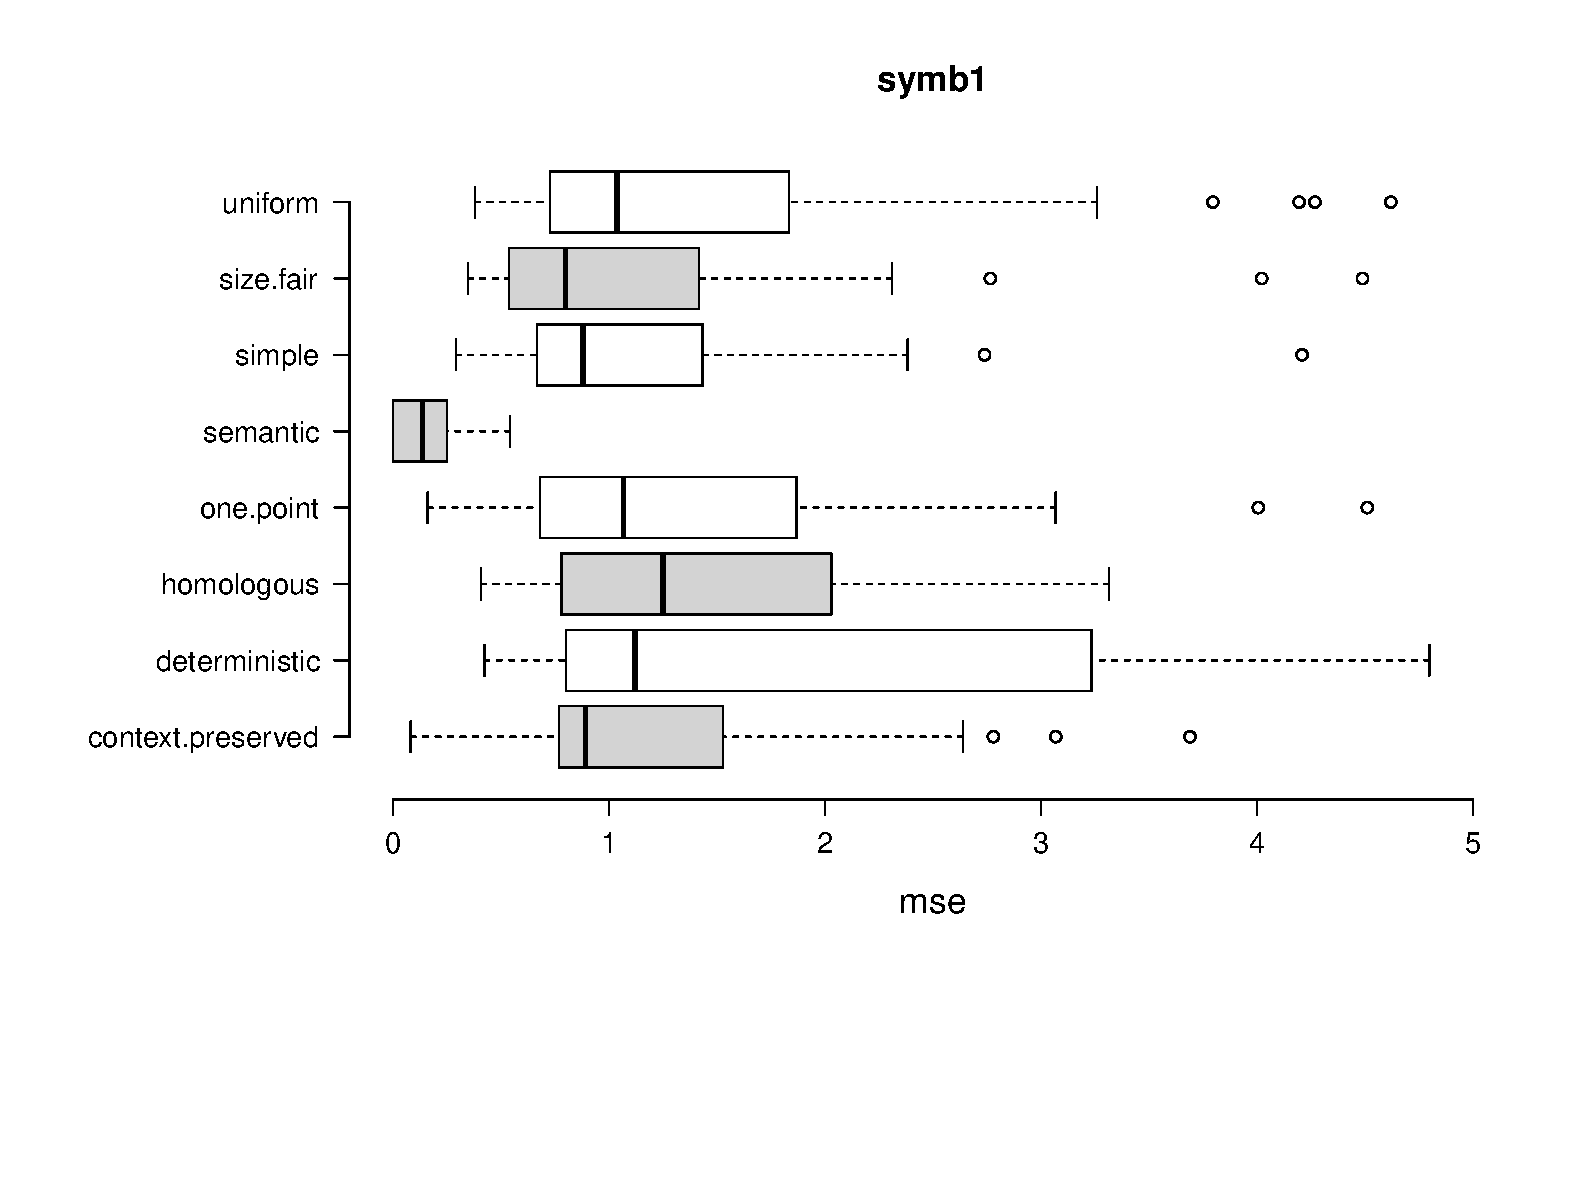
\includegraphics[trim=4cm 5.5cm 0cm 3.5cm, scale=0.3]{./boxPlots/symb1.eps}
\end{figure}

\endminipage
\minipage{0.59\textwidth}
\scalebox{0.59}{
    \centering   
    \begin{tabular}{| l | l | l |}
    \hline
    \textbf{operator} & \textbf{medijan mse-a} & \textbf{rang}\\ \hline
    simple & 0.8796885 & 3\\ \hline
    one point & 1.06746 & 6\\ \hline
    context preserved & 0.8924265 & 4\\ \hline
    size fair & 0.7988625 & 2\\ \hline
    uniform & 1.038325 & 5\\ \hline
    homologous & 1.25174 & 8\\ \hline
    deterministic & 1.120405 & 7\\ \hline
    probabilistic & 18.16455 & 9\\ \hline
    semantic & 0.1364575 & 1\\ \hline
    \end{tabular} 
}
\endminipage
\end{figure}

\begin{itemize}
\item{izraz: $log(x+1)+log(x^2+1)$, $x \in [0, 20]$}
\item{veličina populacije = 400}
\item{broj generacija = 200}
\item{faktor mutacije = 0.5}
\item{nezavršni znakovi: \textit{log, +, -, *}}
\item{završni znakovi: \textit{x, 1}}
\end{itemize}
\end{frame}

%----------------------------------------------------------------------------------------
%	FRAME
%----------------------------------------------------------------------------------------
\begin{frame}
\frametitle{Simbolička regresija 2 (minimizacija)}


\begin{figure}[!htb]
\minipage{0.63\textwidth}
\begin{figure}[H]
	\centering
	\includegraphics[trim=3.5cm 5.5cm 0cm 3.5cm, scale=0.3]{./boxPlots/symb2.eps}
\end{figure}

\endminipage
\minipage{0.59\textwidth}
\scalebox{0.59}{
    \centering   
    \begin{tabular}{| l | l | l |}
    \hline
    \textbf{operator} & \textbf{medijan mse-a}  & \textbf{rang}\\ \hline
    simple & 0 & 1\\ \hline
    one point & 8.07678 & 8\\ \hline
    context preserved & 4.02037 & 5\\ \hline
    size fair & 0 & 1\\ \hline
    uniform & 4.6308 & 7\\ \hline
    homologous & 4.02037 & 5\\ \hline
    deterministic &2.66101 & 4\\ \hline
    probabilistic & 12.3481 & 9\\ \hline
    semantic & 0 & 1\\ \hline
    \end{tabular}
}
\endminipage
\end{figure}

\begin{itemize}
\item{izraz: $sin(x) + sin(y^2)$, $x, y \in [-10, 10]$}
\item{veličina populacije = 100}
\item{broj generacija = 50}
\item{faktor mutacije = 0.2}
\item{nezavršni znakovi: \textit{sin, *, +, -, /}}
\item{završni znakovi: \textit{x, y}}
\end{itemize}
\end{frame}

%----------------------------------------------------------------------------------------
%	FRAME
%----------------------------------------------------------------------------------------
\begin{frame}
\frametitle{Simbolička regresija 3 (minimizacija)}

\begin{figure}[!htb]
\minipage{0.66\textwidth}
\begin{figure}[H]
	\centering
	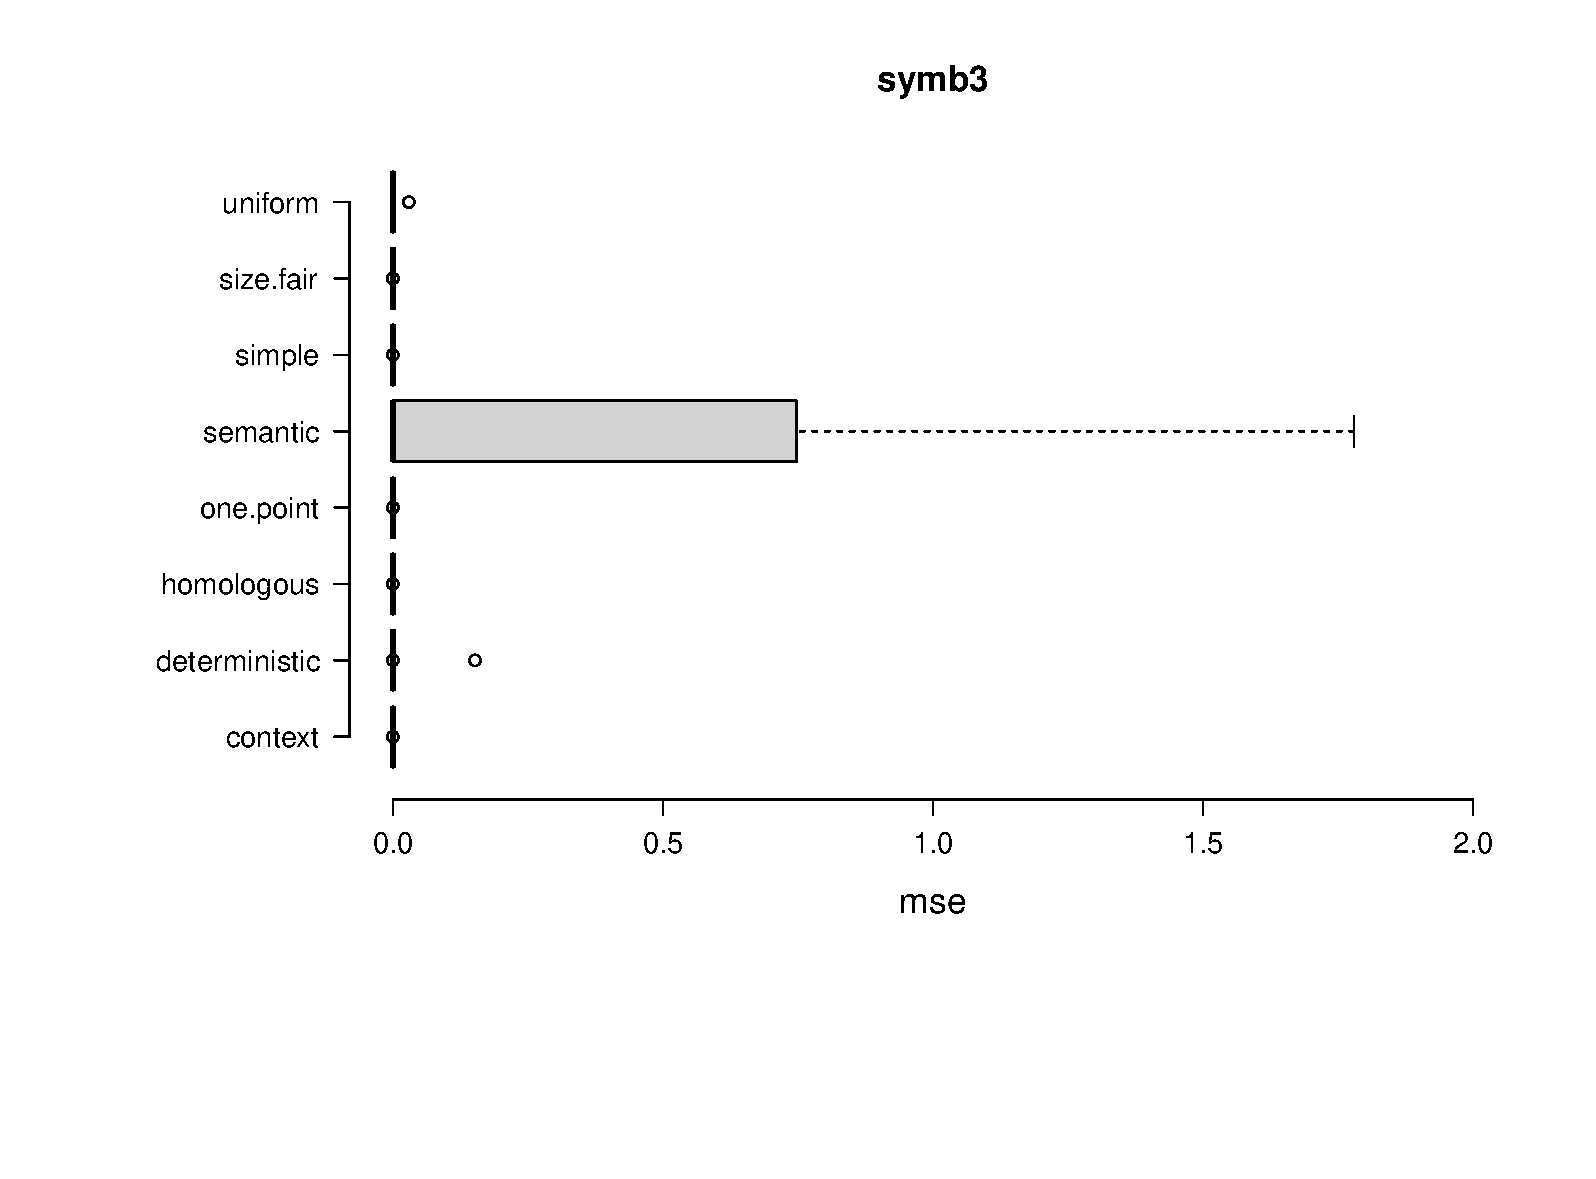
\includegraphics[trim=4cm 5.5cm 0cm 3.2cm, scale=0.3]{./boxPlots/symb3.eps}
\end{figure}

\endminipage
\minipage{0.59\textwidth}
\scalebox{0.59}{
    \centering   
    \begin{tabular}{| l | l | l |}
    \hline
    \textbf{operator} & \textbf{medijan mse-a} & \textbf{rang}\\ \hline
    simple & $7.77 \cdot 10^{-16}$ & 1\\ \hline
    one point & $7.77 \cdot 10^{-16}$ & 1\\ \hline
    context preserved &$7.77 \cdot 10^{-16}$& 1 \\ \hline
    size fair & $7.77 \cdot 10^{-16}$ & 1\\ \hline
    uniform & $7.77 \cdot 10^{-16}$ & 1\\ \hline
    homologous & $7.77 \cdot 10^{-16}$ & 1\\ \hline
    deterministic & $7.77 \cdot 10^{-16}$ & 1\\ \hline
    probabilistic & $7.77 \cdot 10^{-16}$ & 1\\ \hline
    semantic & $1.39 \cdot 10^{-15}$ & 9\\ \hline
    \end{tabular}
    
}
\endminipage
\end{figure}

\begin{itemize}
\item{izraz: $2 \cdot sin(x) \cdot cos(y)$, $x, y \in [-10, 10]$}
\item{veličina populacije = 400}
\item{broj generacija = 50}
\item{faktor mutacije = 0.3}
\item{nezavršni znakovi: \textit{sin, cos, *, +, -, /}}
\item{završni znakovi: \textit{x, y, 2}}
\end{itemize}
\end{frame}

%----------------------------------------------------------------------------------------
%	FRAME
%----------------------------------------------------------------------------------------
\begin{frame}
\frametitle{Simbolička regresija 4 (minimizacija)}


\begin{figure}[!htb]
\minipage{0.63\textwidth}
\begin{figure}[H]
	\centering
	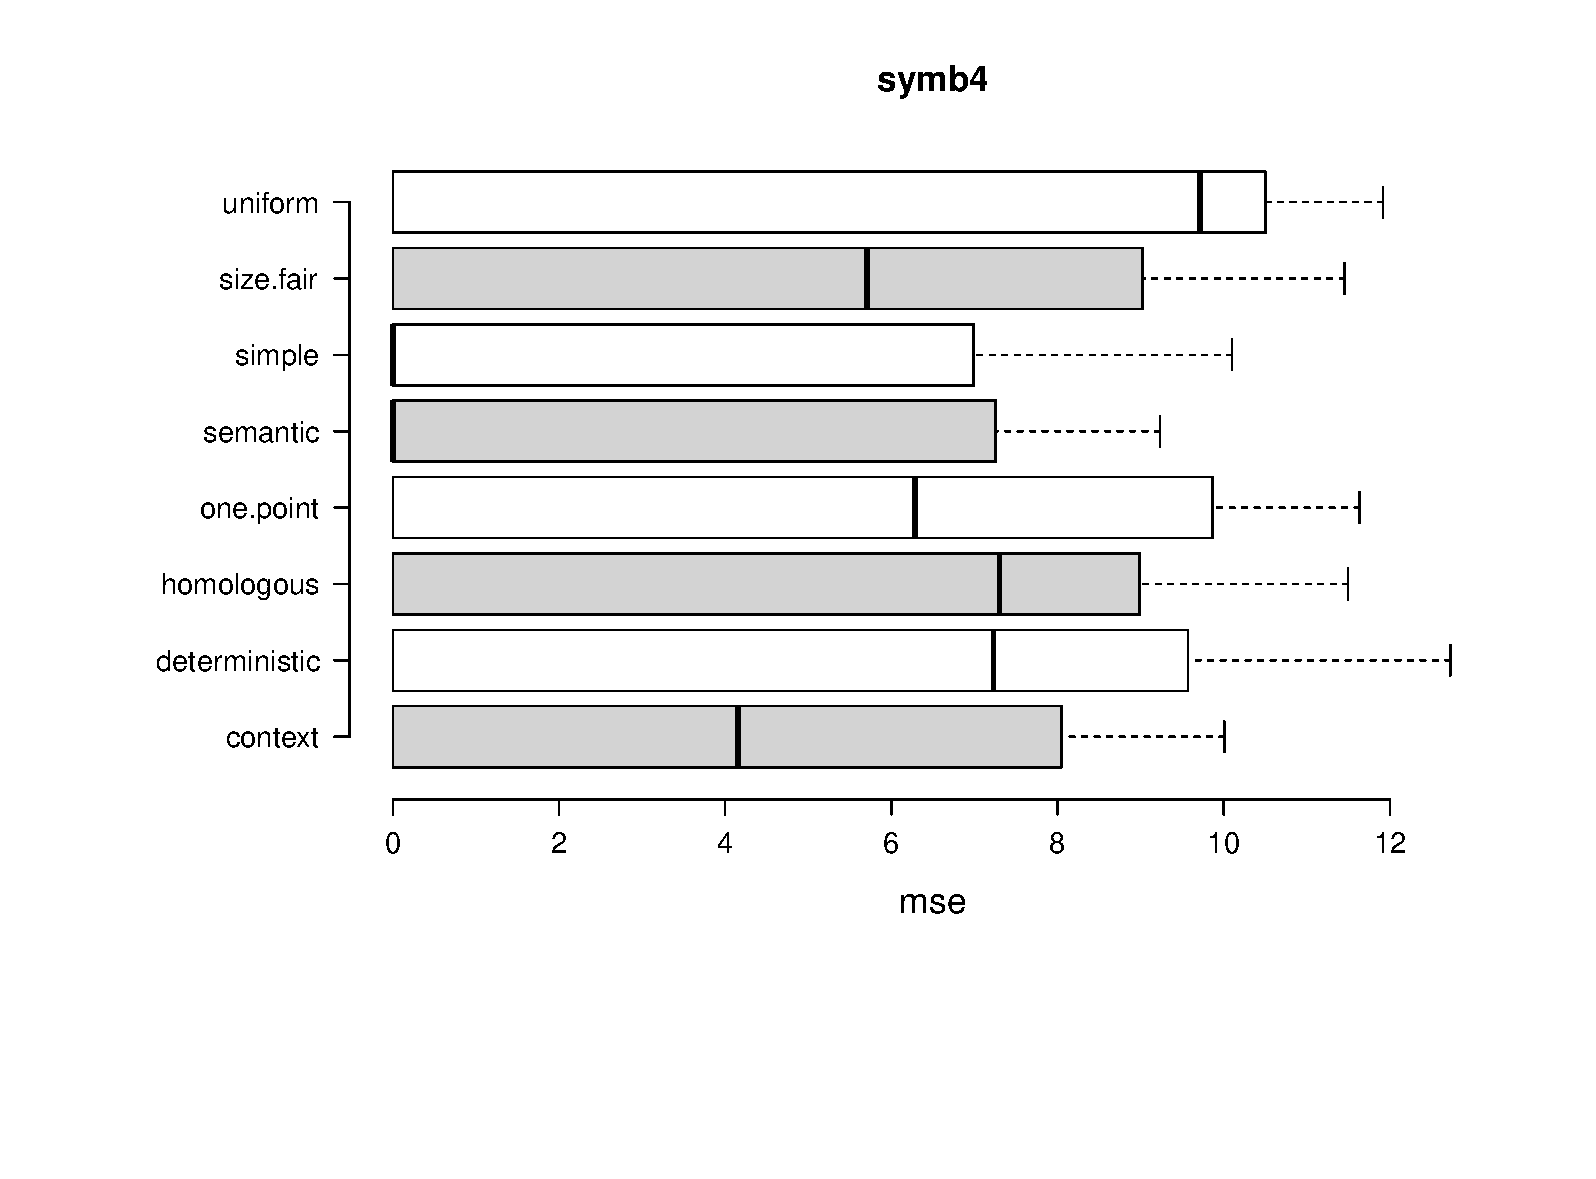
\includegraphics[trim=4cm 5.5cm 0cm 3.5cm, scale=0.3]{./boxPlots/symb4.eps}
\end{figure}

\endminipage
\minipage{0.59\textwidth}
\scalebox{0.59}{
    \centering   
    \begin{tabular}{| l | l | l |}
    \hline
    \textbf{operator} & \textbf{medijan mse-a} & \textbf{rang}\\ \hline
    simple & 0 & 1\\ \hline
    one point & 6.284285 & 5\\ \hline
    context preserved & 4.151965 & 3\\ \hline
    size fair & 5.709685 & 4\\ \hline
    uniform & 9.716085 & 8\\ \hline
    homologous & 7.300545 & 7\\ \hline
    deterministic & 7.22765 & 6\\ \hline
    probabilistic & 12.7275 & 9\\ \hline
    semantic & 0 & 1\\ \hline
    \end{tabular}
    
}
\endminipage
\end{figure}

\begin{itemize}
\item{izraz: $x \cdot y + sin((x+1) \cdot (y-1))$, $x, y \in [-10, 10]$}
\item{veličina populacije = 500}
\item{broj generacija = 200}
\item{faktor mutacije = 0.2}
\item{nezavršni znakovi: \textit{sin, *, +, -, /}}
\item{završni znakovi: \textit{x, y, 1}}
\end{itemize}
\end{frame}

%----------------------------------------------------------------------------------------
%	FRAME
%----------------------------------------------------------------------------------------
\begin{frame}
\frametitle{Simbolička regresija 5 (minimizacija)}


\begin{figure}[!htb]
\minipage{0.65\textwidth}
\begin{figure}[H]
	\centering
	\includegraphics[trim=4cm 5.5cm 0cm 3.5cm, scale=0.3]{./boxPlots/symb5.eps}
\end{figure}

\endminipage
\minipage{0.59\textwidth}
\scalebox{0.59}{
    \centering   
    \begin{tabular}{| l | l | l |}
    \hline
    \textbf{operator} & \textbf{medijan mse-a} & \textbf{rang}\\ \hline
    simple & 0 & 1\\ \hline
    one point & 0 & 1\\ \hline
    context preserved & $2.22 \cdot 10^{-16}$& 8\\ \hline
    size fair & 0 & 1\\ \hline
    uniform & 0 & 1\\ \hline
    homologous & 0 & 1\\ \hline
    deterministic & 0 & 1\\ \hline
    probabilistic & 7.45469 & 9\\ \hline
    semantic & 0 & 1\\ \hline
    \end{tabular}
    
}
\endminipage
\end{figure}

\begin{itemize}
\item{izraz: $\frac{8}{2 + x^2 + y^2}$ , $x, y \in [-10, 10]$}
\item{veličina populacije = 500}
\item{broj generacija = 200}
\item{faktor mutacije = 0.4}
\item{nezavršni znakovi: \textit{+, -, *, /}}
\item{završni znakovi: \textit{x, y, 2, 8}}
\end{itemize}
\end{frame}

%----------------------------------------------------------------------------------------
%	FRAME
%----------------------------------------------------------------------------------------
\begin{frame}
\frametitle{Simbolička regresija 6 (minimizacija)}


\begin{figure}[!htb]
\minipage{0.65\textwidth}
\begin{figure}[H]
	\centering
	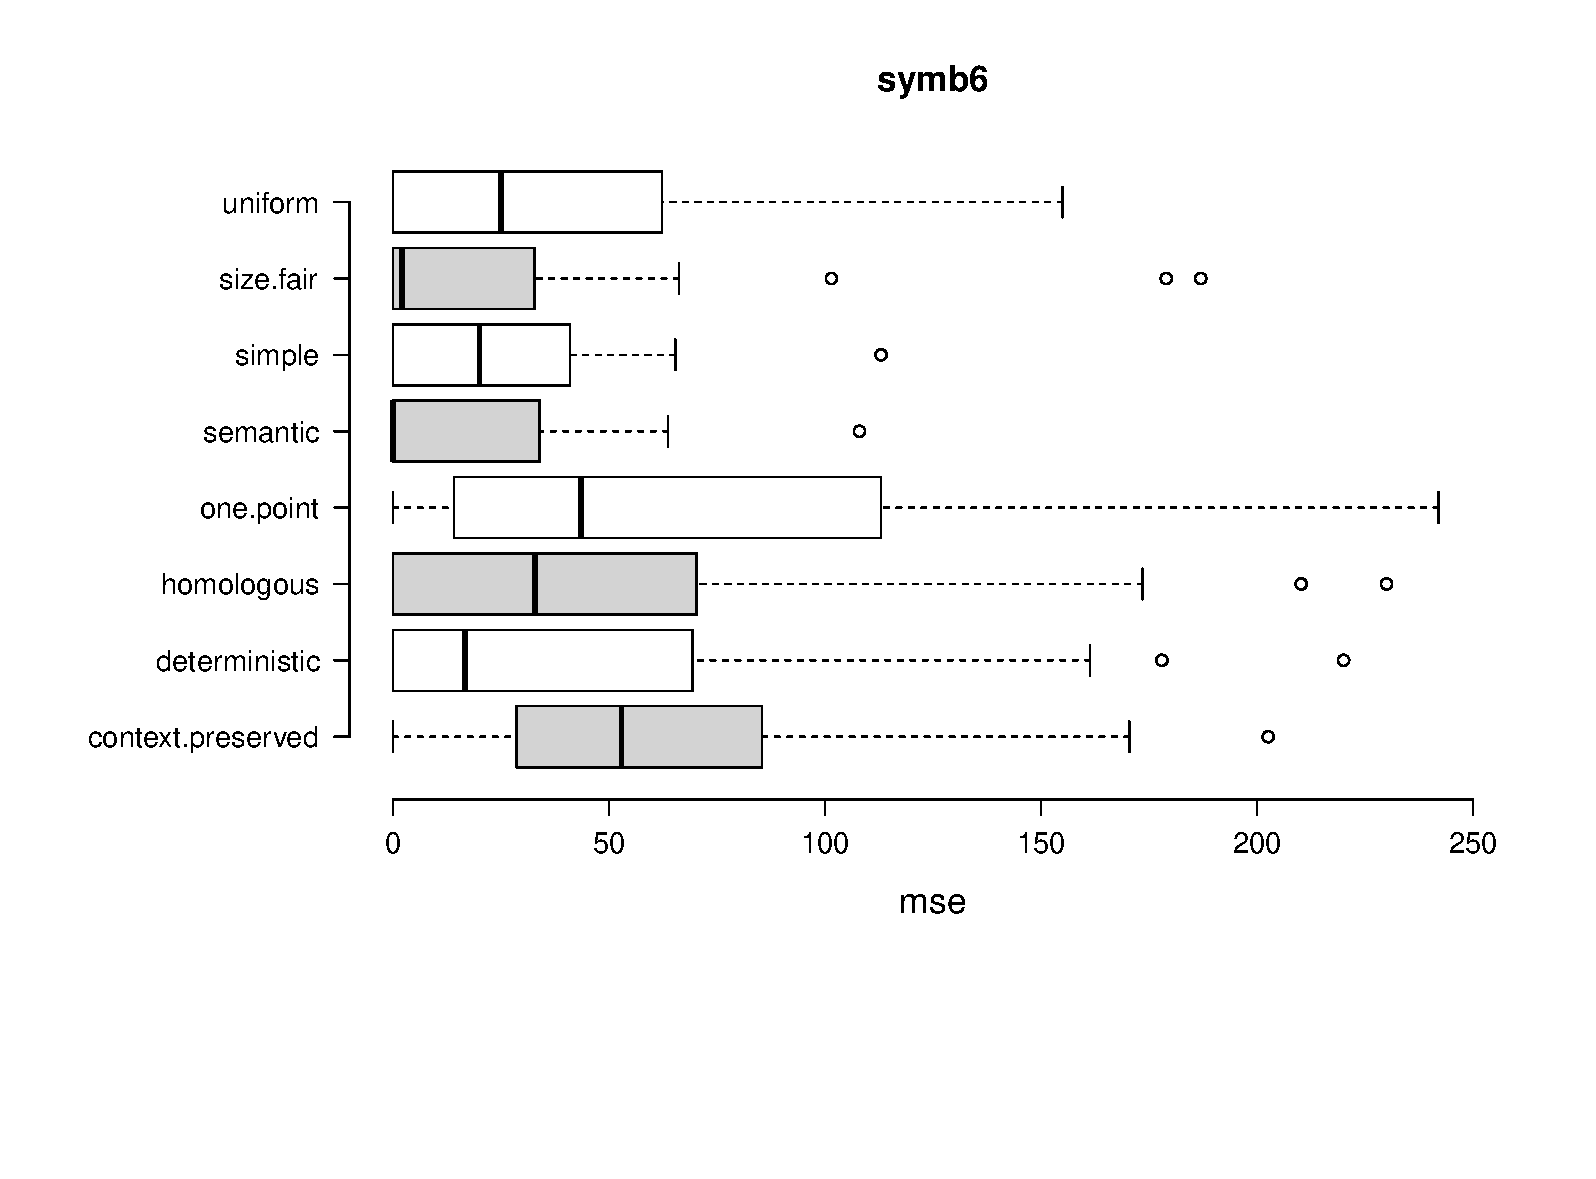
\includegraphics[trim=4cm 5.5cm 0cm 3.5cm, scale=0.3]{./boxPlots/symb6.eps}
\end{figure}

\endminipage
\minipage{0.59\textwidth}
\scalebox{0.59}{
    \centering   
    \begin{tabular}{| l | l | l |}
    \hline
    \textbf{operator} & \textbf{medijan mse-a} & \textbf{rang}\\ \hline
    simple & 20.1 & 4\\ \hline
    one point & 43.6 & 7\\ \hline
    context preserved & 52.9 & 8\\ \hline
    size fair & 2.13 & 2\\ \hline
    uniform & 25 & 5\\ \hline
    homologous & 32.9 & 6\\ \hline
    deterministic & 16.7 & 3\\ \hline
    probabilistic & 1080 & 9\\ \hline
    semantic & $1.18 \cdot 10^{-13}$ & 1\\ \hline
    \end{tabular}
    
}
\endminipage
\end{figure}


\begin{itemize}
\item{izraz: $\frac{x^3}{5} + \frac{y^3}{2} - x - y$ , $x, y \in [-10, 10]$}
\item{veličina populacije = 300}
\item{broj generacija = 200}
\item{faktor mutacije = 0.4}
\item{nezavršni znakovi: \textit{+, -, *, /}}
\item{završni znakovi: \textit{x, y, 2, 5}}
\end{itemize}
\end{frame}

%----------------------------------------------------------------------------------------
%	FRAME
%----------------------------------------------------------------------------------------
\begin{frame}
\frametitle{Evolucija funkcije prioriteta za uporabu unutar pravila raspoređivanja (minimizacija)}

\begin{figure}[!htb]
\minipage{0.63\textwidth}
\begin{figure}[H]
	\centering
	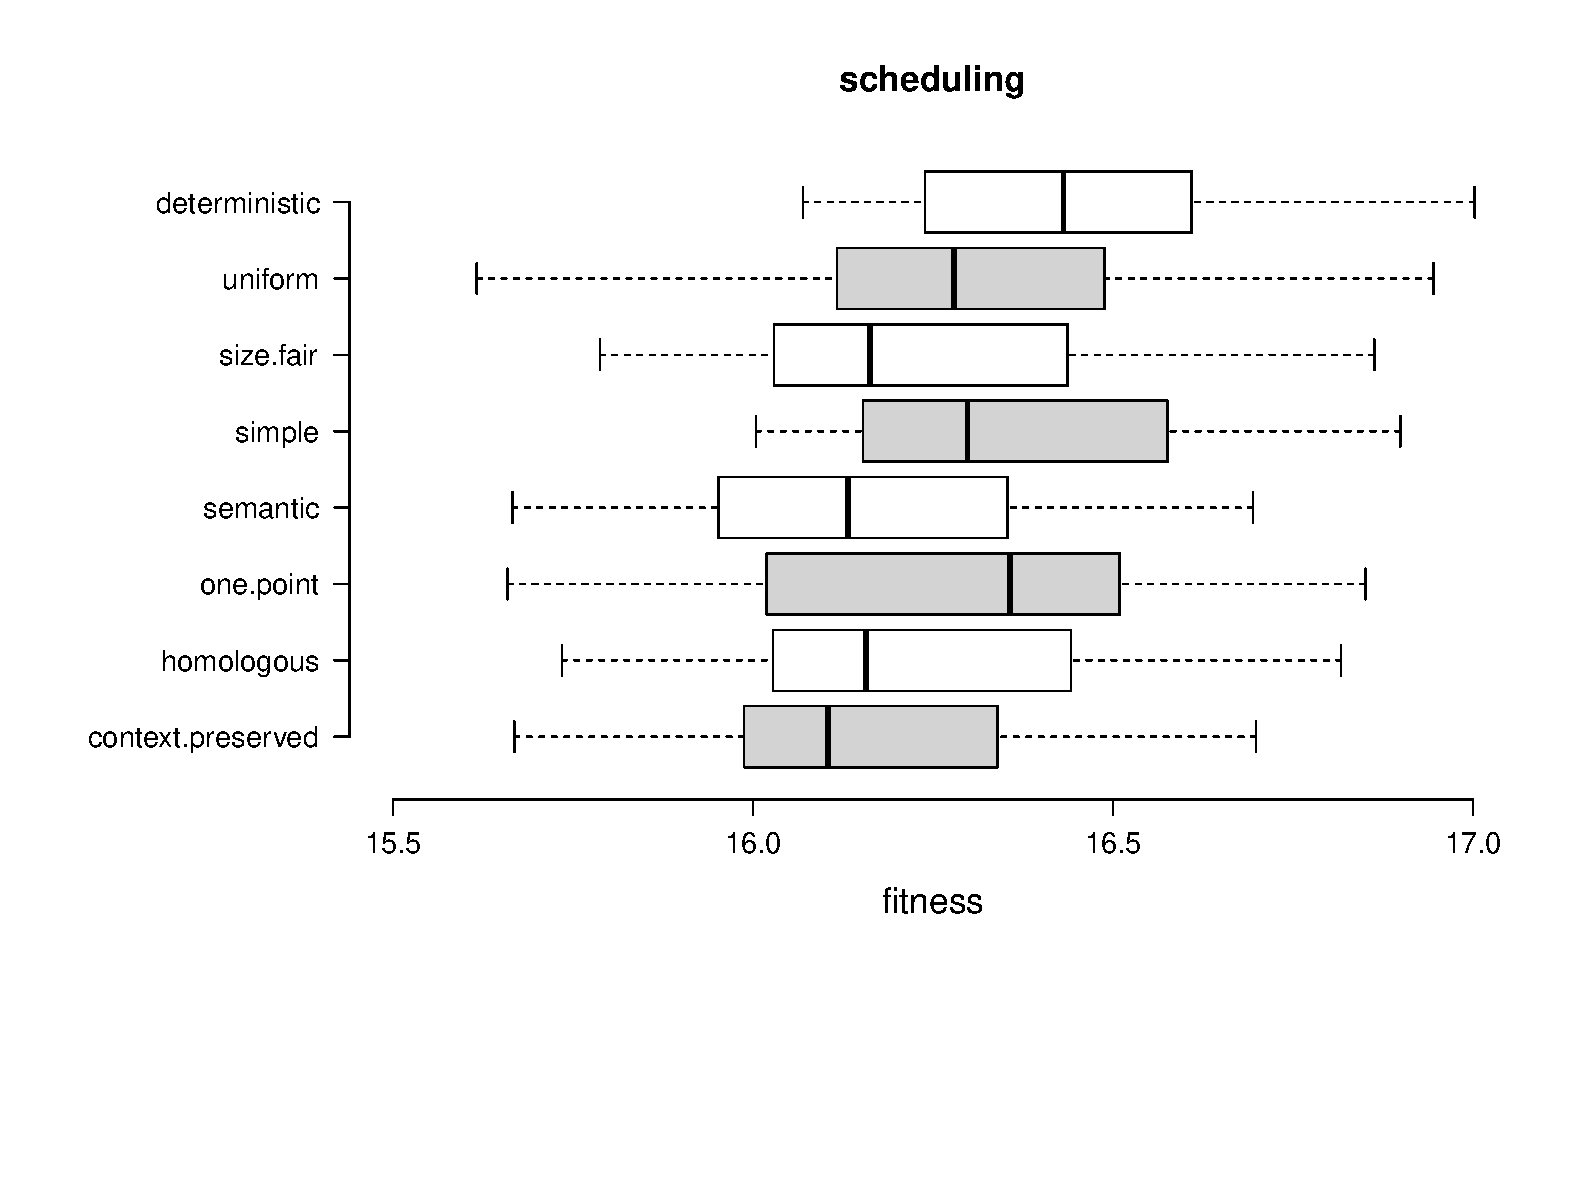
\includegraphics[trim=3.5cm 5.5cm 0cm 3.5cm, scale=0.3]{./boxPlots/iprojekt.eps}
\end{figure}

\endminipage
\minipage{0.59\textwidth}
\scalebox{0.59}{
    \centering   
    \begin{tabular}{| l | l | l |}
    \hline
    \textbf{operator} & \textbf{medijan dobrote} & \textbf{rang}\\ \hline
    simple & 16.2982 & 6\\ \hline
    one point & 16.2566 & 7\\ \hline
    context preserved & 16.1039 & 1\\ \hline
    size fair & 16.16284 & 4\\ \hline
    uniform & 16.2794 & 5\\ \hline
    homologous & 16.1527 & 3\\ \hline
    deterministic & 16.4313 & 8\\ \hline
    probabilistic & 21.30655 & 9\\ \hline
    semantic & 16.13225 & 2\\ \hline
    \end{tabular}
    
}
\endminipage
\end{figure}

\begin{itemize}
\item{veličina populacije = 500}
\item{broj generacija = 30}
\item{faktor mutacije = 0.3}
\item{nezavršni znakovi: \textit{+, -, *, /, pos}}
\item{završni znakovi: \textit{pt, dd, w, SL, pmin, pavg, PAT, MR, age}}
\end{itemize}
\end{frame}

%----------------------------------------------------------------------------------------
%	FRAME
%----------------------------------------------------------------------------------------
\begin{frame}
\frametitle{Problem umjetnoga mrava (maksimizacija)}


\begin{figure}[!htb]
\minipage{0.63\textwidth}
\begin{figure}[H]
	\centering
	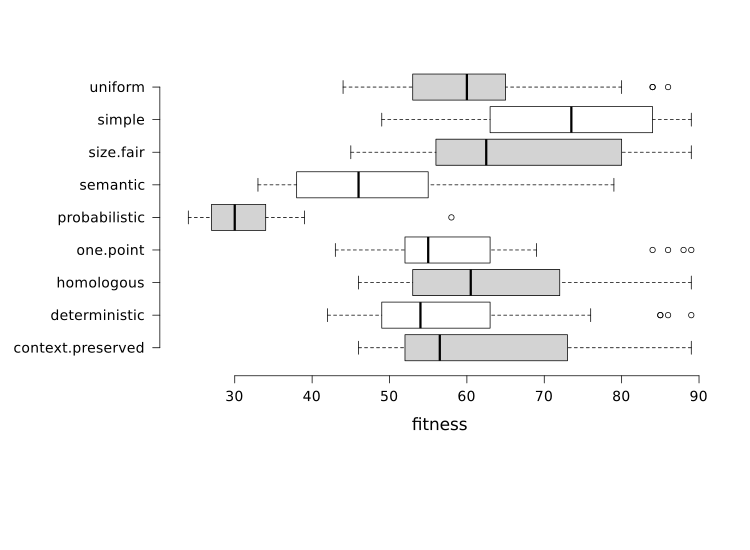
\includegraphics[trim=3cm 5.5cm 0cm 3.5cm, scale=0.3]{./boxPlots/ant.eps}
\end{figure}

\endminipage
\minipage{0.59\textwidth}
\scalebox{0.59}{
    \centering   
    \begin{tabular}{| l | l | l |}
    \hline
    \textbf{operator} & \textbf{medijan dobrote} & \textbf{rang}\\ \hline
    simple & 68.5 & 1\\ \hline
    one point & 55 & 7\\ \hline
    context preserved & 56.5 & 6\\ \hline
    size fair & 62.5 & 3\\ \hline
    uniform & 60 & 5\\ \hline
    homologous & 60.5 & 4\\ \hline
    semantic & 65 & 2\\ \hline
    \end{tabular}
    
    
}
\endminipage
\end{figure}

\begin{itemize}
\item{veličina populacije = 400}
\item{broj generacija = 100}
\item{faktor mutacije = 0.4}
\item{nezavršni znakovi: \textit{Prog2, Prog3, IfFoodAhead}}
\item{završni znakovi: \textit{left, right, move}}
\end{itemize}
\end{frame}

%----------------------------------------------------------------------------------------
%	FRAME
%----------------------------------------------------------------------------------------
\begin{frame}
\frametitle{Sveukupni rezultati}
\begin{itemize}
\item{rangovi operatora za sve probleme - prosječan rang, ukupan prosječan rang i medijani ranga}
\end{itemize}
\begin{table}[H]
 	\centering
    \begin{tabular}{| l | l | l | l |}
    \hline
   \textbf{operator} & \textbf{prosječan} & \textbf{ukupan prosječan}
    & \textbf{medijan} \\ \hline
   simple & 2.0833 & 1 & 1\\ \hline
   one point & 5.5 & 8 & 6\\ \hline
   context preserved & 4.1667 & 4 & 4.5\\ \hline
   size fair & 2.25 & 2 & 2\\ \hline
   uniform & 4.4167 & 7 & 5\\ \hline
   homologous & 4.1667 & 4 & 4.5\\ \hline
   deterministic & 4.2857 & 6 & 4\\ \hline
   probabilistic & 7.8571 & 9 & 9\\ \hline
   semantic & 2.8333 & 3 &  1\\ \hline

 
    \end{tabular}
\end{table}
\end{frame}

\section{Zaključak}

%----------------------------------------------------------------------------------------
%	FRAME
%----------------------------------------------------------------------------------------
\begin{frame}
\frametitle{Zaključak}
\begin{itemize}
\item{u većini slučajeva, najučinkovitije jednostavno križanje i njegova kombinacija sa semantičkim u omjeru 9:1}
\item{dosta dobro pokazalo se i križanje pravedno s obzirom na veličinu}
\item{križanje s jednom točkom prekida pokazalo se kao dosta loše, unatoč svojoj širokoj upotrebi}
\item{jednostavno križanje pokazalo se kao vrlo sigurna polazišna točka u odabiru operatora križanja}
\end{itemize}

\end{frame}
\end{document}
